% Working report based on the supplied DA241O final term paper template.
% Overleaf main document: main.tex. Compile with pdfLaTeX.
% Unfinished sections retain the template's instructional placeholders.
% The explicit page breaks before References and the back matter reproduce
% the supplied template; remove/adapt those breaks when writing the report.
\documentclass[12pt,a4paper]{article}
\usepackage[T1]{fontenc}
% Latin Modern follows the Computer Modern typography of Assignments 1 and 2.
\usepackage{lmodern}
\usepackage{microtype}
\usepackage{graphicx}
\usepackage{amsmath}
\usepackage{booktabs}
\usepackage{enumitem}
\usepackage{float}
\usepackage{csquotes}
\usepackage[backend=biber,style=apa,sorting=nyt]{biblatex}
\addbibresource{airline_references.bib}
\graphicspath{{figures/}}
\newcommand{\HHI}{\textnormal{\textsc{hhi}}}
\newcommand{\objref}[1]{O#1}
\newcommand{\sourcenote}[1]{\par\smallskip{\footnotesize\textit{Source:} #1}}
\usepackage[section]{placeins}
\usepackage{caption}
\captionsetup[figure]{font=small,labelfont=bf,justification=raggedright,singlelinecheck=false,skip=7pt}
\usepackage[margin=1in]{geometry}
\usepackage{setspace}
\onehalfspacing
\setlength{\parindent}{0pt}
\setlength{\parskip}{6pt}
\usepackage{titlesec}
\titleformat{\section}{\large\bfseries}{\thesection.}{0.6em}{}
\titleformat{\subsection}{\normalsize\bfseries}{\thesubsection}{0.6em}{}
\titlespacing*{\section}{0pt}{1.2em}{0.45em}
\titlespacing*{\subsection}{0pt}{0.85em}{0.3em}
\usepackage{fancyhdr}
\pagestyle{fancy}
\fancyhf{}
\fancyhead[L]{DA241O: Managerial Economics}
\fancyhead[R]{Final Term Paper}
\fancyfoot[C]{\thepage}
\renewcommand{\headrulewidth}{0.4pt}
\setlength{\headheight}{14.5pt}
\addtolength{\headsep}{-2.5pt}
\usepackage[hidelinks]{hyperref}

% The source prints its bullets as ordinary, unindented paragraphs.
\newcommand{\templatebullet}[1]{\par\noindent\textbullet\hspace{5.88pt}#1\par}

\begin{document}
\hypersetup{pageanchor=false}
\begin{titlepage}
\centering
\vspace*{2cm}
{\Large\bfseries DA241O: MANAGERIAL ECONOMICS\par}
\vspace{1.5cm}
{\LARGE\bfseries Final Term Paper\par}
\vspace{1.5cm}
{\Large\bfseries [Title of the Study]\par}
\vspace{2cm}
{\large\textbf{Team Name:} [Team Name]\par}
\vspace{0.75cm}
{\large\textbf{Team Members:}\par}
\vspace{0.3cm}
{\large Name 1\\
Name 2\\
Name 3\\
Name 4\par}
\vfill
{\large DA241O: Managerial Economics\\
Department / Programme\\
Date of Submission\par}
\end{titlepage}
\hypersetup{pageanchor=true}
\setcounter{page}{1}

\section*{Abstract}
Briefly present the research problem, research question, data and methodology, main findings, and key implications.

\vspace{0.5cm}
\textbf{Keywords:} [Keyword 1]; [Keyword 2]; [Keyword 3]; [Keyword 4]

\section{Introduction}
\subsection{Background and Problem Statement}
Introduce the market, firm, sector, or policy setting being studied and explain the problem being investigated.

\subsection{Research Question}
State the primary research question.

\subsection{Research Objectives}
State the 2--3 research objectives.

\textbf{O2.} Which groups absorbed Jet Airways' and Go First's passengers and capacity, and how much the Tata consolidation raised concentration through common ownership alone, read against CCI's combination order.

\subsection{Economic Framework}
Identify the economic concept or framework used in the study and explain its relevance to the research question.

Examples may include demand and supply, market structure, information asymmetry, adverse selection, network effects, opportunity cost, principal-agent problems, or other relevant concepts from the course.

\subsection{Scope of the Study}
Specify the relevant market, geography, time period, population, firms, products, or other boundaries of the study.

\section{Literature Review}
\subsection{Existing Literature}
Review the relevant academic, government, industry, and other credible sources.

\subsection{Synthesis of Literature}
Discuss the major findings, patterns, and differences across the literature.

\subsection{Research Gap}
Clearly identify what is not adequately addressed by the existing literature and how the present study addresses this gap.

\subsection{Relevance to the Present Study}
Explain how the existing literature and identified gap inform the research question and analysis.

\section{Data and Methodology}
\subsection{Research Design}
Briefly describe the research design used in the study.

\subsection{Data Sources}
Describe the data source or sources, period covered, geographic coverage, sample or number of observations where applicable, and data collection procedure where applicable.

\subsection{Unit of Analysis}
Clearly identify the unit of analysis, such as firm, product, transaction, household, district, city, industry, or another relevant unit.

\subsection{Variables and Measures}
Define the key variables, indicators, measures, or categories used in the analysis.

For quantitative studies, identify the dependent variable, main explanatory variables, and relevant control variables where applicable.

\subsection{Method of Analysis}
Explain the analytical method used and why it is appropriate for the research question and data.

\textbf{O2.} For each exit, every ownership group's average passenger and seat-km share is compared over up to 12 months before and after, excluding the exit month. A group's absorption share is its gain as a percentage of the exiting airline's previous share, and its contribution is how much that gain raised \HHI{}. For each Tata step, the rise in \HHI{} from common ownership alone, with no passengers switching airline, is compared with the change actually observed, and the result is read against CCI's combination order \parencite{cci2023vistara}. This accounting answers the objective's question directly: who gained, and how much each gain raised concentration. Full workings are in Appendix~\ref{app:workings}.

Examples may include:
\templatebullet{Descriptive analysis}
\templatebullet{Comparative analysis}
\templatebullet{Regression analysis}
\templatebullet{Market concentration measures}
\templatebullet{Price analysis}
\templatebullet{Index construction}
\templatebullet{Cost-benefit analysis}
\templatebullet{Cost-effectiveness analysis}
\templatebullet{Case analysis}
\templatebullet{Qualitative analysis}

\subsection{Hypotheses or Expected Relationships}
State the hypotheses or expected relationships developed during the research process, where applicable.

\begin{itemize}[leftmargin=2em]
	\item \textbf{H3 (O2):} IndiGo has the largest absorption ratio after both exits, larger after Go First.
	\item \textbf{H4 (O2):} IndiGo's gain accounts for over half of the \HHI{} rise after each exit.
\end{itemize}

% Keep the first O4 description and figure together in this working draft.
\clearpage
\section{Descriptive and Exploratory Analysis}
\subsection{O2: Exits and Tata consolidation}
\textbf{Exits: exploratory analysis.} Neither exit was sudden (Figure~\ref{fig:o2-exits}). Jet Airways' passenger share fell from 16.2\% to 5.7\% in the year before its April 2019 exit, and Go First's from 11.1\% to 6.4\% in the year before its May 2023 exit, as both grounded aircraft. Some traffic therefore moved before the exit month, so the before-window already includes part of the shift and the before-and-after comparison may understate it. IndiGo rose most around both exits, from about 43\% to 48\% after Jet Airways and from about 57\% to 62\% after Go First. The market grew in both post-exit windows, with passengers rising faster than seat-km, so rivals mainly filled existing seats (Table~\ref{tab:o2-market}). Section~\ref{sec:o2-results} uses these before-and-after windows to measure how much of each exiting airline's share every group absorbed.

\begin{figure}[H]
\centering
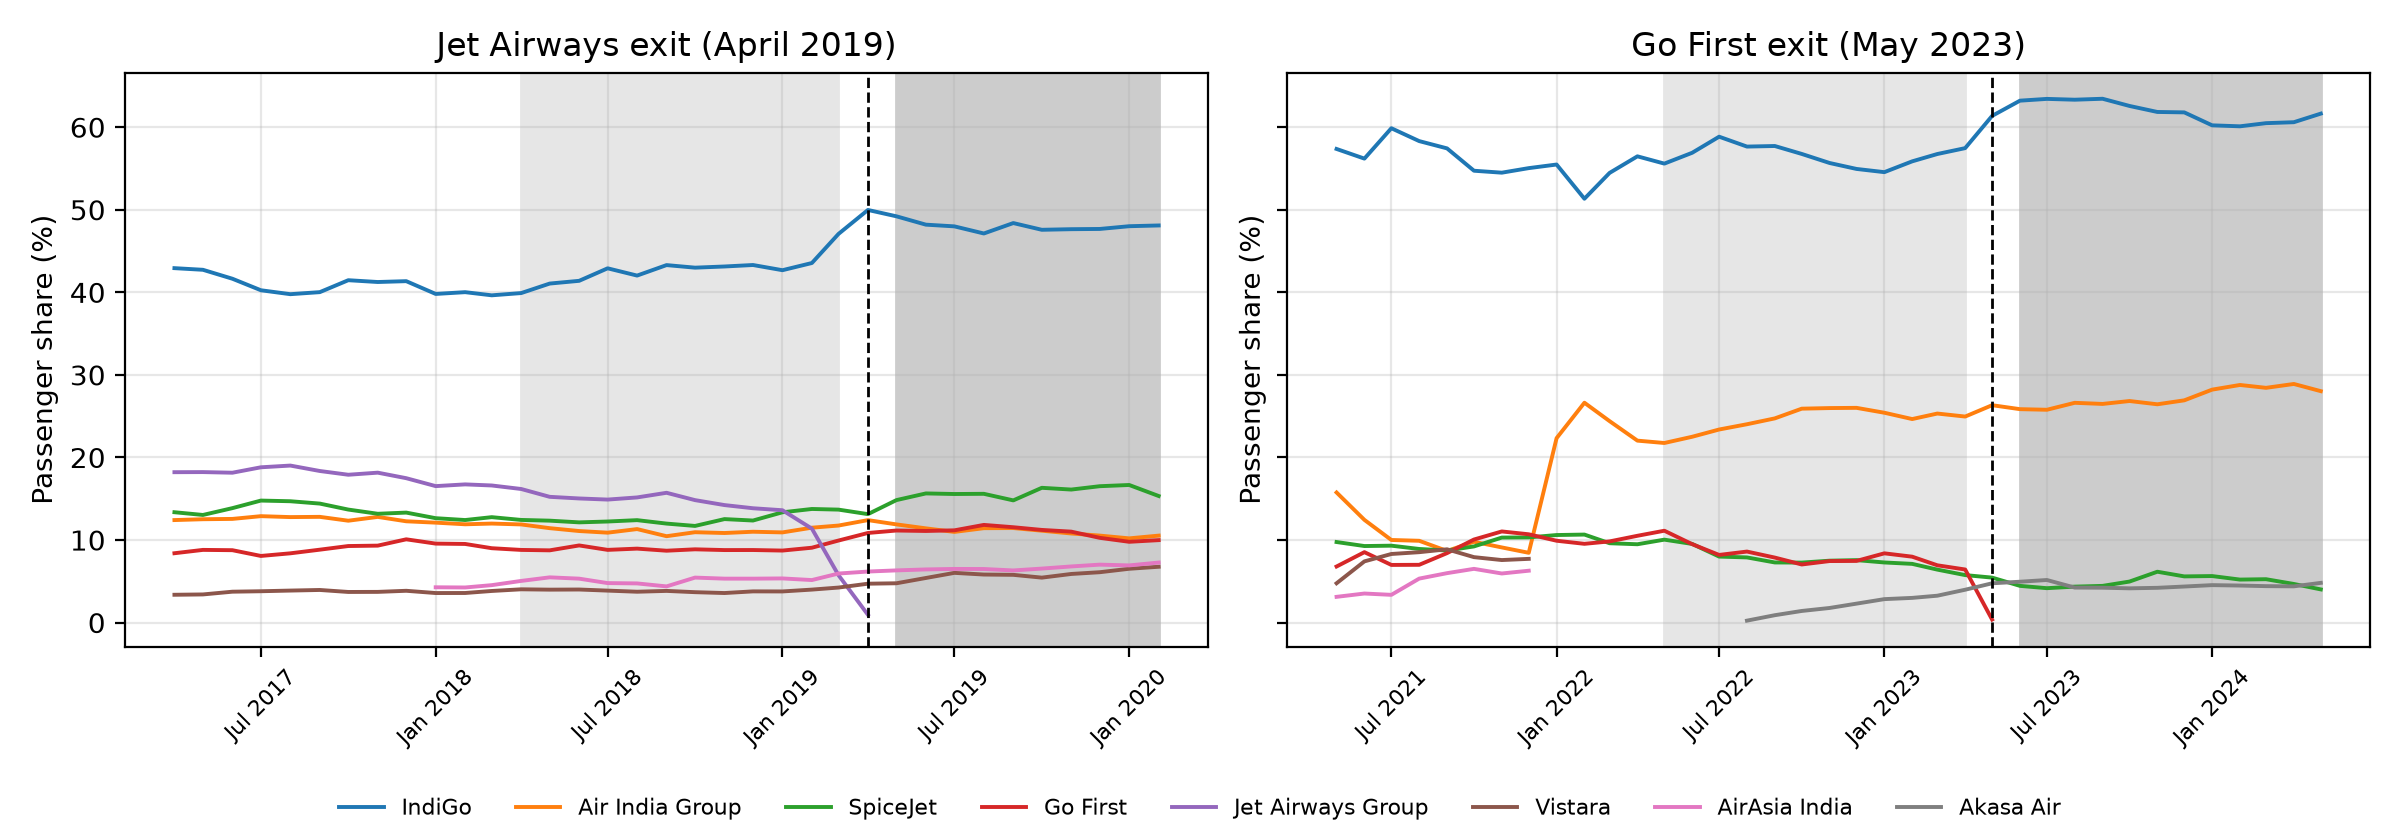
\includegraphics[width=\textwidth]{o2_exit_share_paths.png}
\caption{Monthly passenger shares by ownership group around the Jet Airways and Go First exits}\label{fig:o2-exits}
\sourcenote{DGCA monthly airline statistics via \textcite{kubicek2026aviationstats}; authors' calculations. Light shading: 12-month pre-exit window; dark shading: post-exit window (10 months for Jet Airways, ending before COVID-19); dashed line: exit month, excluded from both windows. The Air India Group's jump in January 2022 is the Tata acquisition grouping, not an exit effect.}
\end{figure}

\begin{table}[H]
\centering
\caption{Market size and capacity before and after each exit (monthly averages)}\label{tab:o2-market}
\small
\begin{tabular}{@{}llrrrr@{}}
\toprule
Exit & Window & \shortstack[r]{Passengers\\(million)} & \shortstack[r]{Capacity\\(billion seat-km)} & \shortstack[r]{Load\\factor (\%)} & \shortstack[r]{Groups\\$\geq$1\% share} \\
\midrule
Jet Airways & Apr 2018--Mar 2019 & 11.69 & 13.07 & 86.0 & 8.0 \\
 & May 2019--Feb 2020 & 12.25 & 13.60 & 87.1 & 7.0 \\
Go First & May 2022--Apr 2023 & 11.53 & 13.29 & 84.1 & 5.6 \\
 & Jun 2023--May 2024 & 12.88 & 14.25 & 87.2 & 4.6 \\
\bottomrule
\end{tabular}
\sourcenote{DGCA monthly airline statistics via \textcite{kubicek2026aviationstats}; authors' calculations. Capacity (seat-km) $=$ seats offered $\times$ kilometres flown. Load factor $= 100 \times \dfrac{\text{passenger-km}}{\text{seat-km}}$, the share of seats filled.}
\end{table}

\textbf{Tata consolidation: descriptive analysis.} The brands brought under one owner in January 2022 held 22.5\% of passengers, and those merged in late 2024 held 29.3\% (Table~\ref{tab:o2-tata}). These shares are the inputs to the mechanical \HHI{} calculation in Section~\ref{sec:o2-results}.

\begin{table}[H]
\centering
\caption{Passenger shares of the Tata brands before each consolidation step (\%)}\label{tab:o2-tata}
\small
\begin{tabular}{@{}lrrrrr@{}}
\toprule
Step (shares in) & Air India & AI Express & Vistara & AirAsia India\textsuperscript{a} & Total \\
\midrule
Acquisition, Jan 2022 (Dec 2021) & 8.39 & 0.07 & 7.72 & 6.28 & 22.46 \\
Mergers, Dec 2024 (Sep 2024) & 11.14 & 3.97 & 10.04 & 4.11 & 29.26 \\
\bottomrule
\end{tabular}
\sourcenote{DGCA monthly airline statistics via \textcite{kubicek2026aviationstats}; authors' calculations. \textsuperscript{a}Renamed AIX Connect. September 2024 is the last month before the AIX Connect merger (October 2024) and the Vistara merger (November 2024).}
\end{table}

\subsection{O4: National concentration trends}
Figure~\ref{fig:o4-national-eda} summarises 138 observed months from January 2015 to July 2026. The two largest ownership groups' combined passenger share (CR2) rises from 60.7\% to 91.3\%, while their share gap increases from 12.5 to 43.4 percentage points. The leading pair is IndiGo and Jet Airways Group in January 2015, and IndiGo and Air India Group in July 2026; groups are ranked afresh each month.

The January 2022 movement includes the study's inclusion of Vistara and AirAsia India/AIX Connect in the Air India Group. It should therefore not be attributed entirely to changes in airline passenger volumes. April 2020 is missing and is not interpolated.

\begin{figure}[htbp]
\centering
\IfFileExists{figures/o4_national_cr2_share_gap.pdf}{%
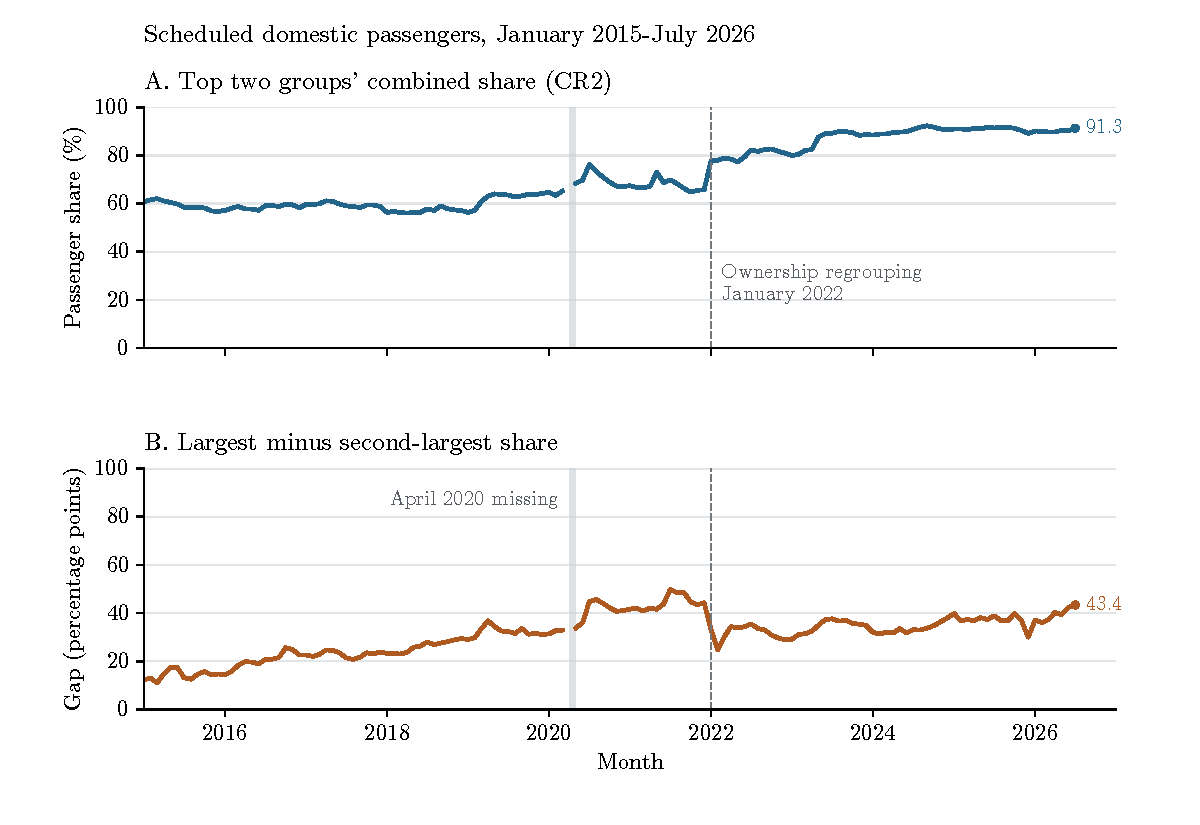
\includegraphics[width=\linewidth]{figures/o4_national_cr2_share_gap.pdf}%
}{\fbox{\parbox[c][4cm][c]{0.9\linewidth}{\centering O4 figure pending: \nolinkurl{figures/o4_national_cr2_share_gap.pdf}}}}
\caption{National concentration and share asymmetry, 2015--2026.}
\label{fig:o4-national-eda}
\vspace{2pt}
\begin{minipage}{\linewidth}
\footnotesize\setstretch{1.1}
\textit{Source:} DGCA monthly traffic via \href{https://github.com/mkubicek/india-aviation-stats/tree/16770ac59dae61ce7b80fd8bd67dd7f4cef280a6}{Kubicek (2026)}; authors' calculations.
\end{minipage}
\end{figure}

\section{Analysis and Results}
Present the main analysis and findings.

The specific form of analysis will depend on the research question and methodology. This section may include statistical results, regression results, calculated measures or indices, comparative results, tables and figures, qualitative findings, or other relevant empirical evidence.

Interpret the results in terms of their economic meaning and relevance to the research question.

\subsection{O2: Who gained from exits and consolidation}\label{sec:o2-results}
\textbf{Who absorbed the exits.} IndiGo had the highest passenger-share absorption after both exits: 37.7\% for Jet Airways and 66.0\% for Go First (Table~\ref{tab:o2-absorption}). After Jet Airways' exit, SpiceJet was second (22.9\%), followed by Vistara, Go First and AirAsia India. After Go First's exit, Akasa Air (35.3\%) and the Air India Group (33.7\%) also gained. Go First was not the only airline losing share: SpiceJet and other airlines also lost share. Adding only the positive absorption percentages gives more than 100\%; including the negative percentages brings the total back to 100\%.

\begin{table}[H]
\centering
\caption{Share of the exiting airline absorbed by each group, and contribution to the change in \HHI{}}\label{tab:o2-absorption}
\small
\begin{tabular}{@{}lrrrrrr@{}}
\toprule
 & \multicolumn{3}{c}{Jet Airways exit (Apr 2019)} & \multicolumn{3}{c}{Go First exit (May 2023)} \\
\cmidrule(lr){2-4}\cmidrule(l){5-7}
Group & Passengers & Seat-km & $c_g$ & Passengers & Seat-km & $c_g$ \\
\midrule
IndiGo & 37.7 & 28.5 & 473 & 66.0 & 66.0 & 632 \\
SpiceJet & 22.9 & 30.4 & 90 & $-$33.7 & $-$36.2 & $-$34 \\
Air India Group & $-$1.0 & 1.5 & $-$3 & 33.7 & 30.3 & 141 \\
Akasa Air & -- & -- & -- & 35.3 & 40.7 & 18 \\
Go First & 14.1 & 11.4 & 39 & -- & -- & -- \\
Vistara & 14.3 & 14.2 & 19 & \multicolumn{3}{c}{in Air India Group} \\
AirAsia India & 10.6 & 13.3 & 17 & \multicolumn{3}{c}{in Air India Group} \\
Others & 1.4 & 0.7 & 0 & $-$1.3 & $-$0.8 & 0 \\
\midrule
Exiting airline removed & & & $-$191 & & & $-$65 \\
Total change in \HHI{} & 100 & 100 & +444 & 100 & 100 & +690 \\
\bottomrule
\end{tabular}
\sourcenote{DGCA monthly airline statistics via \textcite{kubicek2026aviationstats}; authors' calculations. Passengers and Seat-km: absorption $a_g$ (\%), a group's change in mean share divided by the exiting airline's pre-exit mean share. $c_g$: contribution to the change in \HHI{} (points), using passenger shares. Windows: Apr 2018--Mar 2019 vs May 2019--Feb 2020 (Jet Airways); May 2022--Apr 2023 vs Jun 2023--May 2024 (Go First).}
\end{table}

\textbf{Who drove the rise in concentration.} IndiGo's gain alone added 473 \HHI{} points after Jet Airways' exit, more than the total rise of 444, because Jet Airways' own 191 points disappeared. After Go First's exit it added 632 of the 690-point rise (92\%). The seat-km results are similar (IndiGo: 352 of 354 points after Jet Airways; 599 of 653 after Go First).

\textbf{Capacity versus filling seats.} After Jet Airways' exit, SpiceJet took a larger share of Jet Airways' seat-km (30.4\%) than of its passengers (22.9\%), so it expanded capacity. Its annual report confirms that it was allotted 74 of the vacated slots and inducted 31 aircraft made available by the suspension \parencite[p.~62]{spicejet2020annual}. IndiGo did the reverse (28.5\% of seat-km, 37.7\% of passengers), filling seats it already had. After Go First's exit, Akasa Air added capacity (40.7\% of seat-km against 35.3\% of passengers), partly reflecting its own ramp-up since August 2022. Go First's decline was fleet-driven: engine problems had grounded a significant part of its fleet well before the exit \parencite[p.~35]{goair2021drhp}.

\textbf{Tata consolidation.} At the January 2022 acquisition, ownership \HHI{} rose by 373 points against a mechanical rise of 334 from common ownership alone, so almost all of the rise is the ownership effect (Table~\ref{tab:o2-mech}). This comparison is affected by the recovery from COVID-19, as the before-window is all of 2021. At the December 2024 mergers, brand \HHI{} rose by 493 points against a mechanical 256. The gap does not come from the merged group: the Tata brands' combined share fell from 28.3\% to 26.7\%, so their own contribution rose by only about 135 points. Most of the gap is IndiGo's continued growth, from 61.5\% to 64.5\%, which alone added about 380 points. The observed rise was therefore at least the mechanical rise at both steps, but for different reasons. This is an additional check, not stated as a hypothesis in Assignment~2.

\begin{table}[H]
\centering
\caption{Mechanical and observed change in \HHI{} at each Tata consolidation step (points)}\label{tab:o2-mech}
\small
\begin{tabular}{@{}llrrr@{}}
\toprule
Step & Measure & Mechanical & Observed & Difference \\
\midrule
Acquisition (Jan 2022) & Ownership \HHI{} & +334 & +373 & +39 \\
Mergers (Dec 2024) & Brand \HHI{} & +256 & +493 & +237 \\
\bottomrule
\end{tabular}
\sourcenote{DGCA monthly airline statistics via \textcite{kubicek2026aviationstats}; authors' calculations. Mechanical: $2\sum s_a s_b$ over brands combined, using the shares in Table~\ref{tab:o2-tata}. Observed: 12-month mean after minus 12-month mean before (Jan--Dec 2021 vs Jan--Dec 2022; Oct 2023--Sep 2024 vs Dec 2024--Nov 2025, merger months omitted).}
\end{table}

\textbf{CCI's review of the Vistara merger.} The merger needed CCI approval under the combination provisions of the Competition Act (Sections 5--6) \parencite[slide~65]{gandhi2026marketstructure}. CCI defined the relevant market as the origin--destination city pair, not the national market, and found 48 domestic pairs where Air India and Vistara overlapped, with a combined share above 40\% on some of them \parencite[paras.~19, 109--111]{cci2023vistara}. It approved the merger with voluntary commitments, including keeping a minimum capacity on seven domestic routes for up to four years \parencite[paras.~115--118, 126--127]{cci2023vistara}. It did not assess national concentration, which the merger itself raised by 256 points.

\section{Discussion}
Discuss the findings in relation to:
\templatebullet{The research question}
\templatebullet{The economic framework}
\templatebullet{The existing literature}
\templatebullet{The hypotheses or expected relationships}
\templatebullet{The broader context of the study}
Clearly state whether the hypotheses or expected relationships were supported, partially supported, or not supported, where applicable.

\subsection{O2: Economic interpretation}
\textbf{Exits (O2).} Each exit removed a meaningful competitor. Jet Airways' exit raised ownership \HHI{} from about 2,440 to 2,870, equivalent to the market going from 4.1 to 3.5 equal-sized firms; Go First's raised it from about 3,940 to 4,620, from 2.5 to 2.2 equal-sized firms. In a Cournot oligopoly, the industry's average price markup equals \HHI{} divided by the price elasticity of demand \parencite[slide~48]{gandhi2026marketstructure}. With an illustrative elasticity of 1.5, the two exits would raise the markup by about 3.0 and 4.6 percentage points of price. We have no fare data, so these figures show the size of the change in market structure, not observed fare increases.

\textbf{Why IndiGo absorbed most.} IndiGo behaves like a Stackelberg leader: large, irreversible aircraft orders, including a record order for 500 aircraft in June 2023, commit it to capacity that followers cannot match \parencite[slide~52]{gandhi2026marketstructure}. When Go First left a month earlier, IndiGo had the aircraft to take two-thirds of its passengers. Airport slots, which are rationed licences and so a barrier to entry \parencite[slide~29]{gandhi2026marketstructure}, decided who could add capacity: after Jet Airways' exit, the airline that received the vacated slots (SpiceJet) was the one that expanded. Concentration may partly reflect IndiGo's cost leadership rather than weak competition \parencite[slide~8]{gandhi2026marketstructure}; without fare and cost data we cannot separate the two.

\textbf{Tata consolidation and merger review.} Common ownership alone accounts for most of the January 2022 rise, and the December 2024 mergers added 256 points by themselves. CCI reviewed the Vistara merger route by route and protected seven routes with capacity commitments; it did not consider the national rise. The two views complement each other: route remedies protect travellers on specific routes, but national structure, with two groups carrying about 90\% of passengers, also shapes access to airport slots and the market's exposure to disruption at a single airline.

\subsection{O2: Hypotheses revisited}
\begin{itemize}[leftmargin=2em]
	\item \textbf{H3: IndiGo has the largest absorption ratio after both exits, larger after Go First.}\par
	\textbf{Outcome: Partially supported.} IndiGo absorbed the largest share of passengers after both exits, and a larger share after Go First (66.0\%) than after Jet Airways (37.7\%); but after Jet Airways, SpiceJet took more of the seat-km because it received the vacated slots.
	\item \textbf{H4: IndiGo's gain accounts for over half of the \HHI{} rise after each exit.}\par
	\textbf{Outcome: Supported.} IndiGo's gain accounts for more than half of the rise in \HHI{} after both exits, on both measures.
\end{itemize}
Both results match \textcite{grosche2020concentration}, who find that concentration in German air transport rose after Air Berlin's bankruptcy and that the largest group, Lufthansa, became more dominant, as IndiGo did here.

\begin{table}[H]
\centering
\caption{O2 hypotheses and additional check: outcomes}\label{tab:hypotheses}
\small
\begin{tabular}{@{}p{0.08\textwidth}p{0.23\textwidth}p{0.60\textwidth}@{}}
\toprule
No. & Outcome & Evidence \\
\midrule
H3 & Partially supported & Table~\ref{tab:o2-absorption}: largest for passengers (37.7\%, 66.0\%); SpiceJet larger for seat-km after Jet Airways \\
H4 & Supported & Table~\ref{tab:o2-absorption}: 473 of 444; 632 of 690 points \\
Check & Holds at both steps & Observed \HHI{} rise exceeds mechanical rise at both Tata steps (Table~\ref{tab:o2-mech}); not an Assignment 2 hypothesis \\
\bottomrule
\end{tabular}
\end{table}

\section{Implications and Recommendations}
Discuss the implications of the findings for the relevant stakeholders.

Depending on the topic, these may include:
\templatebullet{Firms and managers}
\templatebullet{Consumers}
\templatebullet{Regulators}
\templatebullet{Policymakers}
\templatebullet{Industry participants}
Provide 2--3 specific recommendations where appropriate. Recommendations should follow from the findings of the study.

\begin{enumerate}[leftmargin=2em]
	\item \textbf{For CCI (O2):} in aviation mergers, assess national concentration and airport-slot holdings alongside route overlaps, and publish compliance with route capacity commitments. The Vistara merger alone raised national brand \HHI{} by 256 points, which the route-level review did not consider (Section~\ref{sec:o2-results}).
	\item \textbf{For the Ministry of Civil Aviation and airport operators (O2):} when an airline exits, reallocate its slots with priority for smaller and newer airlines. After Jet Airways' exit, the airline that received the slots was the one that expanded capacity, while IndiGo's share of both exits shows how quickly the largest firm gains otherwise (Section~\ref{sec:o2-results}).
\end{enumerate}

\section{Limitations}
Discuss the important limitations relating to the data, sample, measurement, methodology, analysis, and interpretation.

Where relevant, mention how these limitations could be addressed in future research.

\textbf{O2.} Both exiting airlines declined before they stopped flying, so the before-windows already include part of the shift and the absorption figures may understate it. Other changes overlap the windows: Akasa Air's ramp-up and SpiceJet's decline during the Go First window, and the end of COVID-19 during the January 2022 comparison. The Jet Airways after-window is ten months to avoid the pandemic. The Cournot markups are illustrative, as we have no fare or cost data. CCI's market is the city pair and ours is national, so the two measure different things, and the share triggers in the CCI commitments are redacted.

\section{Conclusion}
Summarise the research question, main findings, key economic interpretation, and main implications.

\newpage
\printbibliography[title={References}]

\newpage
\appendix
\section{Variable Dictionary}
Include the variable dictionary where applicable.

\section{Additional Tables and Figures}
Include additional tables and figures where applicable.

\section{Additional Analysis}\label{app:workings}
Include full regression output, additional calculations, analysis code, or other supporting analysis where applicable.

\subsection*{O2: Exit decomposition and Tata consolidation}
\textbf{A. Airline exits: worked example for Jet Airways and IndiGo.}
The same steps are repeated for every ownership group and for Go First's exit. Shares are entered as percentages: use 42.78, not 0.4278.
\begin{enumerate}[leftmargin=2em]
	\item \textbf{Choose the before and after periods.} Exclude the exit month and use up to 12 months on each side. For Jet, compare April 2018--March 2019 with May 2019--February 2020; the after period stops before the pandemic. For Go First, compare May 2022--April 2023 with June 2023--May 2024.

	\item \textbf{Calculate average market shares.} Each month, divide a group's passengers by total market passengers and multiply by 100. Then average these monthly shares within each period. Before Jet's exit, Jet's average share was 13.82\%; IndiGo's was 42.78\%. After the exit, IndiGo's was 47.99\%.

	\item \textbf{Find how much IndiGo's share increased.}
	\[
	\text{Share gain} = \text{after share} - \text{before share}
	= 47.99 - 42.78 = 5.21\text{ percentage points}.
	\]

	\item \textbf{Express that gain relative to Jet's former share.}
	\[
	\begin{aligned}
	\text{Absorption (\%)} &= 100\times\frac{\text{group's share gain}}{\text{exiting group's average share before exit}}\\
	&= 100\times\frac{5.21}{13.82} = 37.7\%.
	\end{aligned}
	\]
	IndiGo's gain was equivalent to 37.7\% of Jet's former market share. This is a comparison of market shares, not evidence that 37.7\% of Jet's individual passengers switched to IndiGo. Repeat using seat-km instead of passengers to obtain capacity absorption. A negative value means a surviving group lost share; signed absorption values across all survivors sum to 100\%.

	\item \textbf{Calculate IndiGo's contribution to concentration ($c_g$).} \HHI{} adds the squared shares of all groups. Here $c_g$ denotes group $g$'s contribution, matching the column in Table~\ref{tab:o2-absorption}. Therefore, IndiGo's contribution is:
	\[
	c_g = \text{Contribution} = (\text{after share})^2-(\text{before share})^2
	= 47.99^2-42.78^2 \approx 473\text{ points}.
	\]
	The code uses unrounded shares; displayed inputs are rounded. A larger group generally adds more \HHI{} points for the same share gain because its share is squared.

	\item \textbf{Add all contributions, including Jet's disappearance.} Jet's own contribution is $0^2-13.82^2\approx-191$ points. Adding this to all surviving groups' contributions gives about $+444$ points (Table~\ref{tab:o2-absorption}). This is the change in \HHI{} calculated from average shares. It need not equal the change in average monthly \HHI{}, since squaring an average differs from averaging squares.
\end{enumerate}

\textbf{B. Tata consolidation: worked example for January 2022.}
Here the question is how much concentration rises simply because separate groups become one, even if their shares do not change.
\begin{enumerate}[leftmargin=2em]
	\item \textbf{Hold the pre-acquisition shares fixed.} Use December 2021 shares from Table~\ref{tab:o2-tata}: Air India and Air India Express together, 8.46\%; Vistara, 7.72\%; AirAsia India, 6.28\%. Air India and Air India Express were already one ownership group.

	\item \textbf{Compare separate ownership with common ownership.}
	\[
	\begin{aligned}
	\text{Separate contribution} &= 8.46^2+7.72^2+6.28^2,\\
	\text{Combined contribution} &= (8.46+7.72+6.28)^2,\\
	\text{Mechanical rise} &= \text{combined contribution}-\text{separate contribution}\\
	&= 2(8.46\times7.72+8.46\times6.28+7.72\times6.28)\\
	&\approx334\text{ points}.
	\end{aligned}
	\]
	Other groups' shares are unchanged in this calculation, so their contributions cancel out.

	\item \textbf{Compare with the observed change.} Subtract average monthly ownership \HHI{} for January--December 2021 from that for January--December 2022. The observed rise is 373 points; the difference from the mechanical calculation is $373-334=39$ points. This difference includes changes in market shares and the different measurement periods; it is not a causal estimate of the acquisition's effects.
\end{enumerate}

For the late-2024 mergers, repeat the fixed-share calculation using September 2024 brand shares: the mechanical rise is 256 points. Compare average monthly brand \HHI{} in October 2023--September 2024 with December 2024--November 2025: the observed rise is 493 points. The additional squared-average-share breakdown gives Tata brands $+135$, IndiGo $+380$, SpiceJet $-12$ and Akasa Air $+5$. It indicates which brands drove the rise, but is not an exact decomposition of the 493-point change in average monthly \HHI{}.

\textbf{O4 reproduction files.} Data preparation, Python plotting code, numerical tables and run instructions are available in the \href{https://github.com/Goutham7358/Assignment3_Code}{Assignment 3 code repository}.

\section{Survey Questionnaire or Interview Guide}
Include the survey questionnaire or interview guide where applicable.

\newpage
\section*{Methods and Tools Statement}
Provide a short statement covering:
\templatebullet{Data sources used}
\templatebullet{Software or analytical tools used}
\templatebullet{Other relevant tools used in preparing or analysing the study}
\templatebullet{Any AI tool assistance, where applicable}

\section*{Team Member Contributions}
Provide one line for each team member describing their contribution to the project.

This statement is intended only to confirm that all team members have contributed to the project. It is not an individual assessment of the quality or quantity of each member's contribution, and differences in individual contributions will not result in different marks for team members.
\templatebullet{\textbf{[Member 1]:} [Brief description of contribution.]}
\templatebullet{\textbf{[Member 2]:} [Brief description of contribution.]}
\templatebullet{\textbf{[Member 3]:} [Brief description of contribution.]}
\templatebullet{\textbf{[Member 4]:} [Brief description of contribution.]}

\newpage
\section*{General Note}
The final report should be around 8--12 pages, excluding references and appendices. There is no strict maximum page limit; the length should be appropriate to the scope and depth of the study.

The sections and subsections may be adapted according to the nature of the research question, data, and methodology. Not every subsection will be applicable to every project.

The final report should maintain a clear connection between the research question, economic framework, data, methodology, analysis, findings, and implications.
\end{document}
